
\documentclass[12pt]{ociamthesis}  % default square logo 
%\documentclass[12pt,beltcrest]{ociamthesis} % use old belt crest logo
%|\documentclass[12pt,shieldcrest]{ociamthesis} % use older shield crest logo

\usepackage{lipsum}
\usepackage{setspace}

\usepackage{pgfplots, pgfplotstable}
%load any additional packages
\usepackage{amssymb}
\usepackage{amsmath}
\usepackage{url}
\usepackage[toc,page]{appendix}
\usepackage[font={small}]{caption}
\usepackage{subcaption}
%\usepackage{subfig}
\usepackage{subfloat}
\usepackage[usestackEOL]{stackengine}
\usepackage{epigraph}
\usepackage{multirow}
\def\changemargin#1#2{\list{}{\rightmargin#2\leftmargin#1}\item[]}
\let\endchangemargin=\endlist

\usepackage{soul}
\DeclareRobustCommand{\hlgr}[1]{{\sethlcolor{green}\hl{#1}}}
\usepackage[T1]{fontenc}

\usepackage[bottom]{footmisc}
\usepackage[framemethod=tikz]{mdframed}
\usepackage{enumitem}

\usepackage{graphicx}
\graphicspath{{../figures/}}
\DeclareGraphicsExtensions{.pdf,.png, .gif, .jpg}

\usepackage{dirtree}
\renewcommand*\DTstylecomment{\rmfamily\color{red}\textsc}
%\renewcommand{\DTstyle}{\textrm\expandafter\raisebox{-0.3ex}}
\DTsetlength{0.5em}{0.5em}{0.2em}{0.2pt}{0.2pt}
%\setlength{\DTbaselineskip}{2\baselineskip}

\usepackage{tikz-qtree}
\usepackage{forest}
\usepackage{makecell}
\usepackage{xcolor}
\usepackage{colortbl}
\usepackage{fixltx2e}
\usepackage{rotating}
\newcommand{\anything}{\mathbin{\rotatebox[origin=c]{90}{$\lozenge$}}}
\newcommand{\nothing}{\text{\rule{1.5ex}{0.4pt}\;}}
\newcommand{\Sub}{\rule{1ex}{0.4pt}}

\usepackage{array}
\newcolumntype{M}[1]{>{\arraybackslash}m{#1}}
\newcolumntype{N}{@{}m{0pt}@{}}

\usepackage{tikz-dependency}
%\tikzset{/depgraph/.cd,/depgraph/.search also = {/tikz},
%    baseline=-0.6ex, inner sep=-0.1cm, edge horizontal padding=3pt, edge unit distance=1.5ex}

% ========== AUTOMATIC CELL COLOURING =====%
\makeatletter
\newcommand*{\minuscellcolor}{}
\def\minuscellcolor\ignorespaces{%
  % \ignorespaces not really needed, because \@ifnextchar gobbles spaces
  \@ifnextchar-{\cellcolor{red}}{}%
}

\makeatother

% ========== ALGORITHMS CUSTOMIZATION ==== %

\usepackage{algorithm}
\usepackage[noend]{algpseudocode}
\newcommand*\Arg{\textit}
\newcommand*\func{\textsc}

\usepackage{caption}
\makeatletter
\@addtoreset{algorithm}{chapter}% algorithm counter resets every chapter
\makeatother
\renewcommand{\thealgorithm}{\thechapter.\arabic{algorithm}}% Algorithm # is <chapter>.<algorithm>


\newcommand*\Let[2]{\State #1 $\gets$ #2}
\colorlet{kw}{blue}
\colorlet{rd}{red}
\definecolor{com}{rgb}{0,0.6,0}

% redefine keywords
\algrenewcommand\algorithmicfunction{\textcolor{kw}{\textbf{function}}}
\algrenewcommand\algorithmicwhile{\textcolor{kw}{\textbf{while}}}
\algrenewcommand\algorithmicfor{\textcolor{kw}{\textbf{for}}}
\algrenewcommand\algorithmicif{\textcolor{kw}{\textbf{if}}}
\algrenewcommand\algorithmicelse{\textcolor{kw}{\textbf{else}}}
\algrenewcommand\algorithmicend{\textcolor{kw}{\textbf{end}}}
\algrenewcommand\algorithmicreturn{\textcolor{kw}{\textbf{return}}}
\algrenewcommand\algorithmicthen{\textbf{then}}

\algnewcommand\IF{\If}

% new keywords
\algnewcommand\Break{\textbf{\textcolor{kw}{break}}}%
\algnewcommand\Continue{\textcolor{kw}{continue}}%
\algnewcommand\Each{\textbf{\textrm{each }}}%
\algnewcommand\In{\textbf{\textrm{ in }}}%
\algnewcommand\True{\textcolor{rd}{\textbf{true}}}%
\algnewcommand\False{\textcolor{rd}{\textbf{false}}}%
\algnewcommand\Null{\textcolor{rd}{\textbf{null}}}
\algnewcommand\Or{\textbf{or }}

% redefine loops
\algdef{SE}[WHILE]{While}{EndWhile}[1]{\algorithmicwhile\ #1}{\algorithmicend}%
\algdef{SE}[FOR]{For}{EndFor}[1]{\algorithmicfor\ #1}{\algorithmicend}%
\algdef{C}[IF]{IF}{ElsIf}[1]{\algorithmicelse\algorithmicif\ #1}%

% redefine comments
%\algrenewcommand{\algorithmiccomment}[1]{{\color{com}#1}}


% =========== CUSTOM LSTLISTINGS ====== %

\usepackage{listings}
\definecolor{codegreen}{rgb}{0,0.6,0}
\definecolor{codegray}{rgb}{0.5,0.5,0.5}
\definecolor{codepurple}{rgb}{0.58,0,0.82}
\definecolor{backcolour}{rgb}{0.97,0.97,0.97}

\usepackage{inconsolata}
\lstset{
  basicstyle=\ttfamily,
}
 
\lstdefinestyle{mystyle}{
	basicstyle=\footnotesize\ttfamily,
    backgroundcolor=\color{backcolour},   
    commentstyle=\color{codegreen},
    keywordstyle=\color{magenta},
    numberstyle=\tiny\color{codegray},
    stringstyle=\color{codepurple},
    basicstyle=\footnotesize,
    breakatwhitespace=false,         
    breaklines=true,                 
    captionpos=b,                    
    keepspaces=true,                 
    numbers=left,                    
    numbersep=5pt,                  
    showspaces=false,                
    showstringspaces=false,
    showtabs=false,
    frame=lines,                  
    tabsize=2    
}

\colorlet{punct}{red!60!black}
\definecolor{delim}{RGB}{20,105,176}
\definecolor{mypink}{RGB}{221,54,149}
\colorlet{numb}{magenta!60!black}

\newcommand\JSONnumbervaluestyle{\color{blue}}
\newcommand\JSONstringvaluestyle{\color{mypink}}

% switch used as state variable
\newif\ifcolonfoundonthisline

\makeatletter

\lstdefinelanguage{json}
{
	literate=
		{:}{{{\color{punct}{:}}}}{1}
		{,}{{{\color{punct}{,}}}}{1}
		{\{}{{{\color{delim}{\{}}}}{1}
		{\}}{{{\color{delim}{\}}}}}{1}
		{[}{{{\color{delim}{[}}}}{1}
		{]}{{{\color{delim}{]}}}}{1},
	showstringspaces    = false,
	keywords            = {false,true},
	alsoletter          = 0123456789.,
	morestring          = [s]{"}{"},
	stringstyle         = \ifcolonfoundonthisline\JSONstringvaluestyle\fi,
	MoreSelectCharTable =%
		\lst@DefSaveDef{`:}\colon@json{\processColon@json},
	morecomment=[l]{//}
}

\lstdefinelanguage{JavaScript}{
  keywords={typeof, new, true, false, catch, function, return, null, catch, switch, var, if, in, while, do, else, case, break},
  keywordstyle=\color{blue}\bfseries,
  ndkeywords={class, export, boolean, throw, implements, import, this},
  ndkeywordstyle=\color{darkgray}\bfseries,
  identifierstyle=\color{black},
  sensitive=false,
  comment=[l]{//},
  morecomment=[s]{/*}{*/},
  commentstyle=\color{com}\ttfamily,
  stringstyle=\color{red}\ttfamily,
  morestring=[b]',
  morestring=[b]"
}

\lstdefinelanguage{Rules}{
    literate=
		{->}{{{\color{blue}{->}}}}{1}
		{<}{{{\color{red}{<}}}}{1}
		{>}{{{\color{red}{>}}}}{1}
		{_}{{{\color{red}{\_}}}}{1}
		{|}{{{\color{blue}{|}}}}{1},
  identifierstyle=\color{black},
  sensitive=false,
  comment=[l]{//},
  commentstyle=\color{com}\ttfamily
}

\lstdefinelanguage{Rules2}{
    literate=
		{->}{{{\color{blue}{->}}}}{1}
		{_}{{{\color{blue}{\_}}}}{1},
  keywords={SWAP, TAG, WORDS, DT, PRP,POS,IN,MD,NNS,NN,CC,\$,RB,VB,VBD,VBZ,VBG,VBP},
  keywordstyle=\color{red}\bfseries,
  identifierstyle=\color{black},
  sensitive=false,
  comment=[l]{//},
  commentstyle=\color{com}\ttfamily
}

% flip the switch if a colon is found in Pmode
\newcommand\processColon@json{%
  \colon@json%
  \ifnum\lst@mode=\lst@Pmode%
    \global\colonfoundonthislinetrue%
  \fi
}

\lst@AddToHook{Output}{%
  \ifcolonfoundonthisline%
    \ifnum\lst@mode=\lst@Pmode%
      \def\lst@thestyle{\JSONnumbervaluestyle}%
    \fi
  \fi
  %override by keyword style if a keyword is detected!
  \lsthk@DetectKeywords% 
}

% reset the switch at the end of line
\lst@AddToHook{EOL}%
  {\global\colonfoundonthislinefalse}

\makeatother

\lstset{style=mystyle}
\lstset{basicstyle=\footnotesize\ttfamily}

%======= custom overline ====== %
\newcommand{\tolstrut}{%
  \vrule height\dimexpr\fontcharht\font`\A+.7ex\relax width 0pt\relax
}

\DeclareRobustCommand{\ovl}[1]{%
  \ensuremath{\overline{\mbox{\tolstrut#1}}}%
}

%============ BIBLIOGRAPHY AND REFS PACKAGES ========%
\usepackage[numbers]{natbib}
\usepackage{multibib}
\newcites{x}{References}
\newcites{sec}{Background Reading}

%============ for gloss overline ========%
\makeatletter
\newcommand{\OVER}[1]{$\overline{\hbox{#1}}\m@th$}
\makeatother

\newcommand{\TAG}{\textsuperscript}
\newcommand{\SUB}{\textsubscript}

\usepackage{slgloss}

% ========= for table stuff
\newcommand\Tstrut{\rule{0pt}{2.6ex}}       % "top" strut

% ========= for general formatting of text
\newcommand{\tech}{\texttt}

% ============== stuff below is for header\footer
\usepackage{fancyhdr}
\pagestyle{fancy}
\fancyhead{}
\renewcommand{\sectionmark}[1]{\markright{\textit{#1}}}
\renewcommand{\chaptermark}[1]{\markboth{\arabic{chapter}.\ \textsc{#1}}{}}
\fancyhead[LO]{\leftmark}
\fancyhead[RE]{\rightmark}
%\fancyhead[R]{\rightmark}
%\fancyhead[L]{\leftmark}
\fancyhead[LE,RO]{\bfseries\thepage}
%\cfoot{\fancyplain{}{\thepage}}
\cfoot{}

\let\mtcleardoublepage\cleardoublepage
\renewcommand{\cleardoublepage}{\clearpage{\pagestyle{plain}\mtcleardoublepage}}
\makeatletter
\def\@endpart{\vfil\newpage
              \if@twoside
               \if@openright
                \null
                \thispagestyle{plain}%
                \newpage
               \fi
              \fi
              \if@tempswa
                \twocolumn
              \fi}
\makeatother


\begin{document}

\begin{figure}[H]
	\centering
    \includegraphics[scale=0.75]{chapter1/system-overview-light}
    \caption{Conceptual overview of the system}
    \label{fig:sys-overview}
\end{figure}
\begin{figure}
\begin{center}
\Tree [.S
 	   	 [.NP 
			[.\textcolor{blue}{DT} The ] 
			[.\textcolor{blue}{JJ} large ] 
			[.\textcolor{blue}{NN} cat ] 
 	   	 ]
 	   	 [.VP 
 	   	 	[.\textcolor{blue}{VBP} sat ] 
			[.PP 
				[.\textcolor{blue}{IN} on ]
				[.NP 
					[.\textcolor{blue}{DT} the ] 	
					[.\textcolor{blue}{NN} mat ] 			
				]		
			] 	   	 
 	   	 ]
 	 ]
\end{center}
\caption[English sentence syntax tree]{English sentence syntax tree. Blue text represents word Part of Speech tags.}
\label{fig:english-sent}
\end{figure}

\begin{figure}[H]
\begin{center}
\begin{small}
\begin{tabular}{l|M{0.5cm}|M{0.5cm}|M{0.5cm}|M{0.5cm}|M{0.5cm}|M{0.5cm}|M{0.5cm}|M{0.5cm}|M{0.5cm}|N}
		\multicolumn{1}{l}{}& \multicolumn{9}{l}{Maria no \hphantom{a} dio \space una bofetada a \space la \space bruja verde}\\ 
        \cline{2-10}
        Mary & \cellcolor{black} & & & & & & & & \\ [12pt]
        \cline{2-10}
        did & & \cellcolor{black} & & & & & & & \\ [12pt]
        \cline{2-10}
        not & & \cellcolor{black} & & & & & & & \\ [12pt]
        \cline{2-10}
        slap & & & \cellcolor{black} & \cellcolor{black} & \cellcolor{black} & & & & \\ [12pt]
        \cline{2-10}
        the & & & & & & & \cellcolor{black} & & \\ [12pt]
        \cline{2-10}
        green & & & & & & & & & \cellcolor{black} \\ [12pt]
        \cline{2-10}
        witch & & & & & & & & \cellcolor{black} & \\ [12pt]
        \cline{2-10}
    \end{tabular}  
\end{small}
\caption{Word alignment English-Spanish}
\label{table:alignment}
\end{center}
\end{figure}
\begin{figure}
	\centering
    \includegraphics[scale=1]{chapter2/vaquois}
    \caption[Vaquois triangle for Rule-Based MT]{Vaquois triangle for Rule-Based MT; illustration inspired by \url{https://en.wikipedia.org/wiki/Machine_translation}}
    \label{fig:vaquois}
\end{figure}
\begin{figure}[h]
	\centering
    \includegraphics[scale=1]{chapter2/interlingua}
    \caption[Interlingua representation using ZARDOZ]{Interlingua representation using ZARDOZ; }
    \label{fig:zardoz}
\end{figure}

\begin{figure}[H]
\begin{center}
\begin{small}
\begin{tabular}{l|M{0.5cm}|M{0.5cm}|M{0.5cm}|M{0.5cm}|N}
		\multicolumn{1}{l}{}&\multicolumn{4}{l}{\footnotesize YOU CAKE EAT ?}\\ 
        \cline{2-5}
        Did & \cellcolor{black} & & & \\ [12pt]
        \cline{2-5}
        you & \cellcolor{black} & & & \\ [12pt]
        \cline{2-5}
        eat & & & \cellcolor{black} & \\ [12pt]
        \cline{2-5}
        the & & \cellcolor{black} & & \\ [12pt]
        \cline{2-5}
        cake & & \cellcolor{black} & & \\ [12pt]
        \cline{2-5}
        ? & & & & \cellcolor{black} \\ [12pt]
        \cline{2-5}
    \end{tabular}  
\end{small}
\caption{Word alignment English-ASL}
\label{table:sl-alignment}
\end{center}
\end{figure}

\begin{figure}[h]
	\centering
    \includegraphics[scale=0.75]{chapter3/mt-outline}
    \caption{Machine Translation module design}
    \label{fig:mt-outline}
\end{figure}

\begin{figure}[H]
	\centering
    \includegraphics[scale=0.9]{chapter3/lofi}
    \caption{UI Low fidelity prototype}
    \label{fig:lofi}
\end{figure}
\begin{figure}[H]
	\centering
    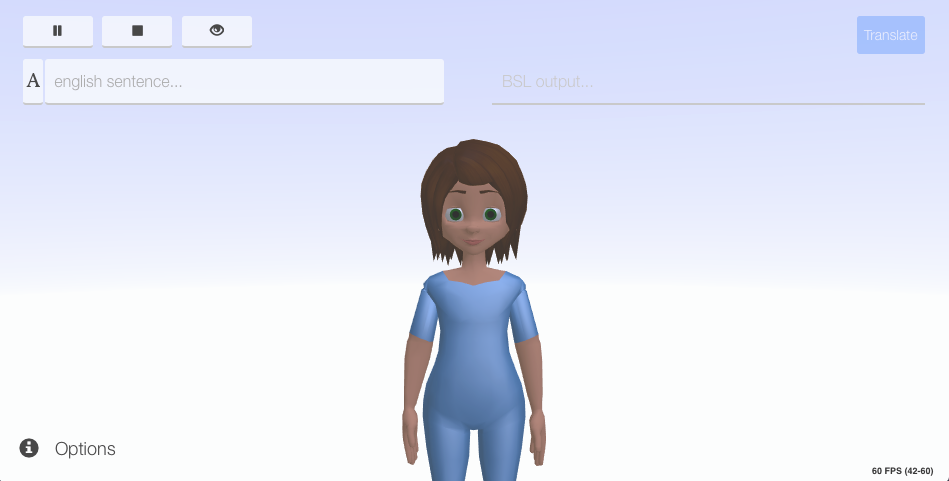
\includegraphics[scale=0.45]{chapter3/full2}
    \caption{UI high fidelity prototype}
    \label{fig:hififull}
\end{figure}


\begin{figure}[H]
	\centering
    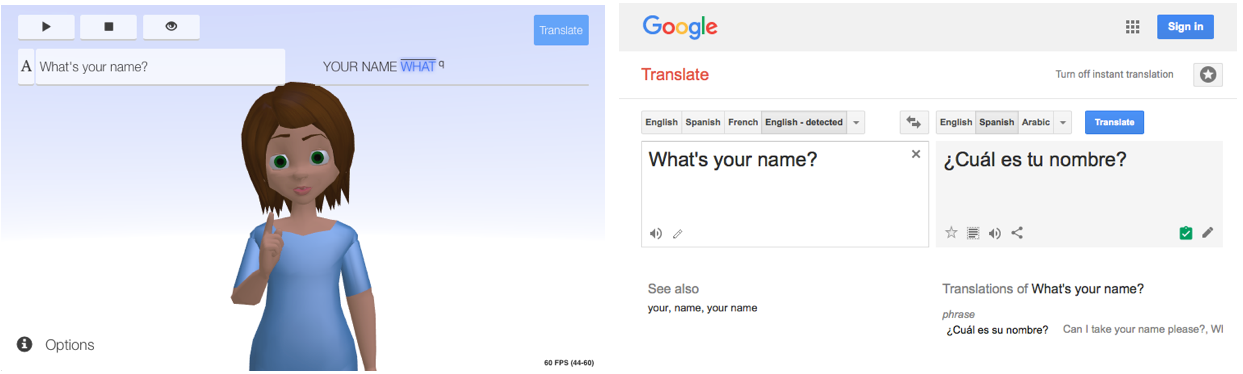
\includegraphics[scale=0.32]{chapter3/compare}
    \caption{UI high fidelity prototype compared to Google Translate}
    \label{fig:hifi}
\end{figure}

\begin{figure}[H]
	\centering
    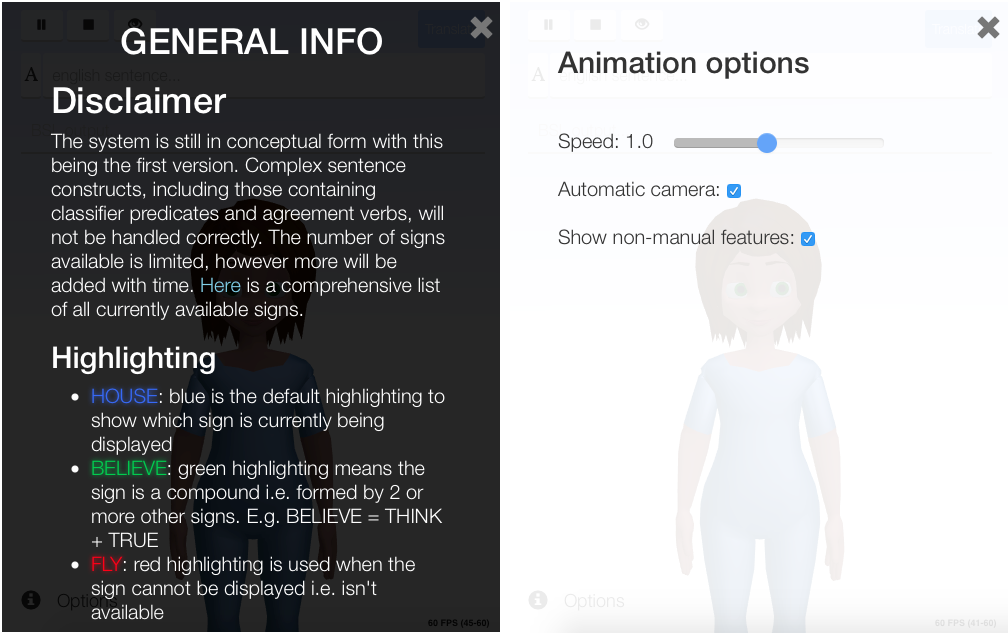
\includegraphics[scale=0.33]{chapter3/info-option}
    \caption{Overlay with additional information and options}
    \label{fig:info-option}
\end{figure}

\begin{figure}[H]
	\centering
    \includegraphics[scale=0.7]{chapter3/flowchart}
    \caption[User interaction flowchart]{User interaction flowchart. Dashed lines show system events and solid lines user actions.}
    \label{fig:flow}
\end{figure}

\begin{figure}[h]
	\centering
    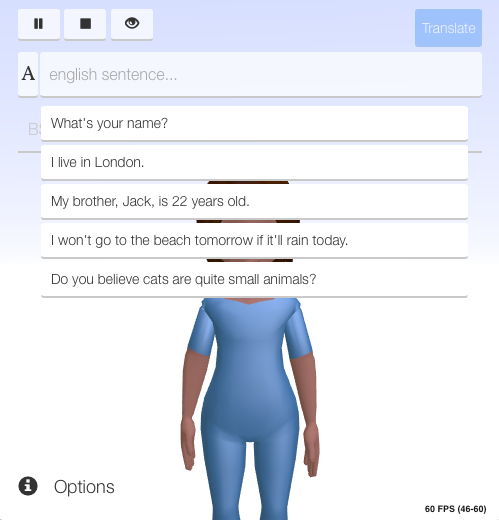
\includegraphics[scale=0.4]{chapter3/suggestions}
    \caption{Sentence suggestions auto-fill}
    \label{fig:suggestions}
\end{figure}

\begin{figure}[h]
	\centering
    \includegraphics[scale=0.8]{chapter4/system-overview-mt}
    \caption{System outline: Machine Translation highlighted}
    \label{fig:sys-over-mt}
\end{figure}	

\begin{figure}[h]
	\centering
    \includegraphics[scale=0.8]{chapter4/mt-objects}
    \caption{Python-side, object oriented overview of the pipeline with transition between sentence representations}
    \label{fig:mt-objects}
\end{figure}	

\begin{figure}[H]
\centering
\begin{subfigure}{.47\textwidth}
  \centering
  \Tree [.NP \edge[red];[.\textcolor{red}{DT} The ] \edge[blue];[.\textcolor{blue}{JJ} big ] \edge[com];[.\textcolor{com}{NNS} cats ] ] 
  \caption{Original syntax tree}
\end{subfigure}%
{\LARGE$\rightarrow$}%
\begin{subfigure}{.47\textwidth}
  \centering
  \Tree [.NP \edge[red];[.\textcolor{red}{DT} The ] \edge[com];[.\textcolor{com}{NNS} cats ] \edge[blue];[.\textcolor{blue}{JJ} big ] ] 
  \caption{Transformed tree}
\end{subfigure}
\caption{Tree transformation using rules: noun phrase}
\label{fig:cat}
\end{figure}

\begin{figure}[H]
\centering
\begin{subfigure}{.47\textwidth}
  \centering
  \Tree [.SQ \edge[red];[.\textcolor{red}{VBP} Have ] \edge[blue];[.\textcolor{blue}{NP} [.PRP you ] ] \edge[blue];[.\textcolor{blue}{VP} [.VBN eaten ] ] ] 
  \caption{}
\end{subfigure}%
{\LARGE$\rightarrow$}%
\begin{subfigure}{.47\textwidth}
  \centering
  \Tree [.SQ \edge[red];[.\textcolor{red}{\vphantom{A}$\nothing$} ] \edge[blue];[.\textcolor{blue}{NP} [.PRP you ] ] \edge[blue];[.\textcolor{blue}{VP} [.VBN eaten ] ] ] 
  \caption{}
\end{subfigure}
\caption{Tree transformation using rules: question}
\label{fig:qtree}
\end{figure}

\begin{figure}[H]
\centering
\begin{subfigure}{.47\textwidth}
  \centering
  \Tree [.SQ
          [.VBP Have ]
          [.NP [.DT the ] [.JJ big ] [.NNS cats ] ]
          [.VP [.VBN eaten ] ] ] 
  \caption{}
\end{subfigure}%
{\LARGE$\rightarrow$}%
\begin{subfigure}{.47\textwidth}
  \centering
  \Tree [.SQ
          [.VBP \vphantom{A}$\nothing$ ]
          [.NP [.DT the ] [.NNS cats ] [.JJ big ] ]
          [.VP [.VBN eaten ] ] ] 
  \caption{}
\end{subfigure}
\caption{Combined example of tree transformation}
\label{fig:cat+q}
\end{figure}

\begin{figure}[H]
\centering
\begin{subfigure}[b]{.5\textwidth}
  \hspace*{-0.5cm}
  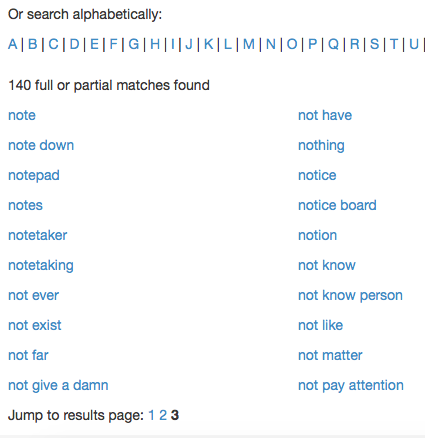
\includegraphics[scale=0.55]{chapter4/signbank}
  \caption{}
\end{subfigure}
\qquad
\begin{subfigure}[b]{.4\textwidth}
  \small
    \begin{lstlisting}[language=Rules,mathescape=true]
about time
above all
...
note down
not ever
not exist
not far
not give a damn
not have
notice board
not know
not know person
not like
not matter
not pay attention
...
worn out
would not
year before
\end{lstlisting}
  \caption{}
\end{subfigure}
\caption{SignBank website data and formatted result}
\label{fig:signbank}
\end{figure}

\begin{figure}[H]
\centering
\includegraphics[scale=0.55]{chapter4/SMI}
\caption{Source Match Indexes derived from the match groups}
\label{fig:smi}
\end{figure}

\begin{figure}[H]
	\centering
    \includegraphics[scale=0.75]{chapter4/system-overview-anim}
    \caption{System outline: Animation Engine highlighted}
    \label{fig:sys-over-anim}
\end{figure}	

\begin{figure}[H]
\centering
\begin{subfigure}[b]{.5\textwidth}
	\captionsetup{width=0.8\textwidth}
  \centering
  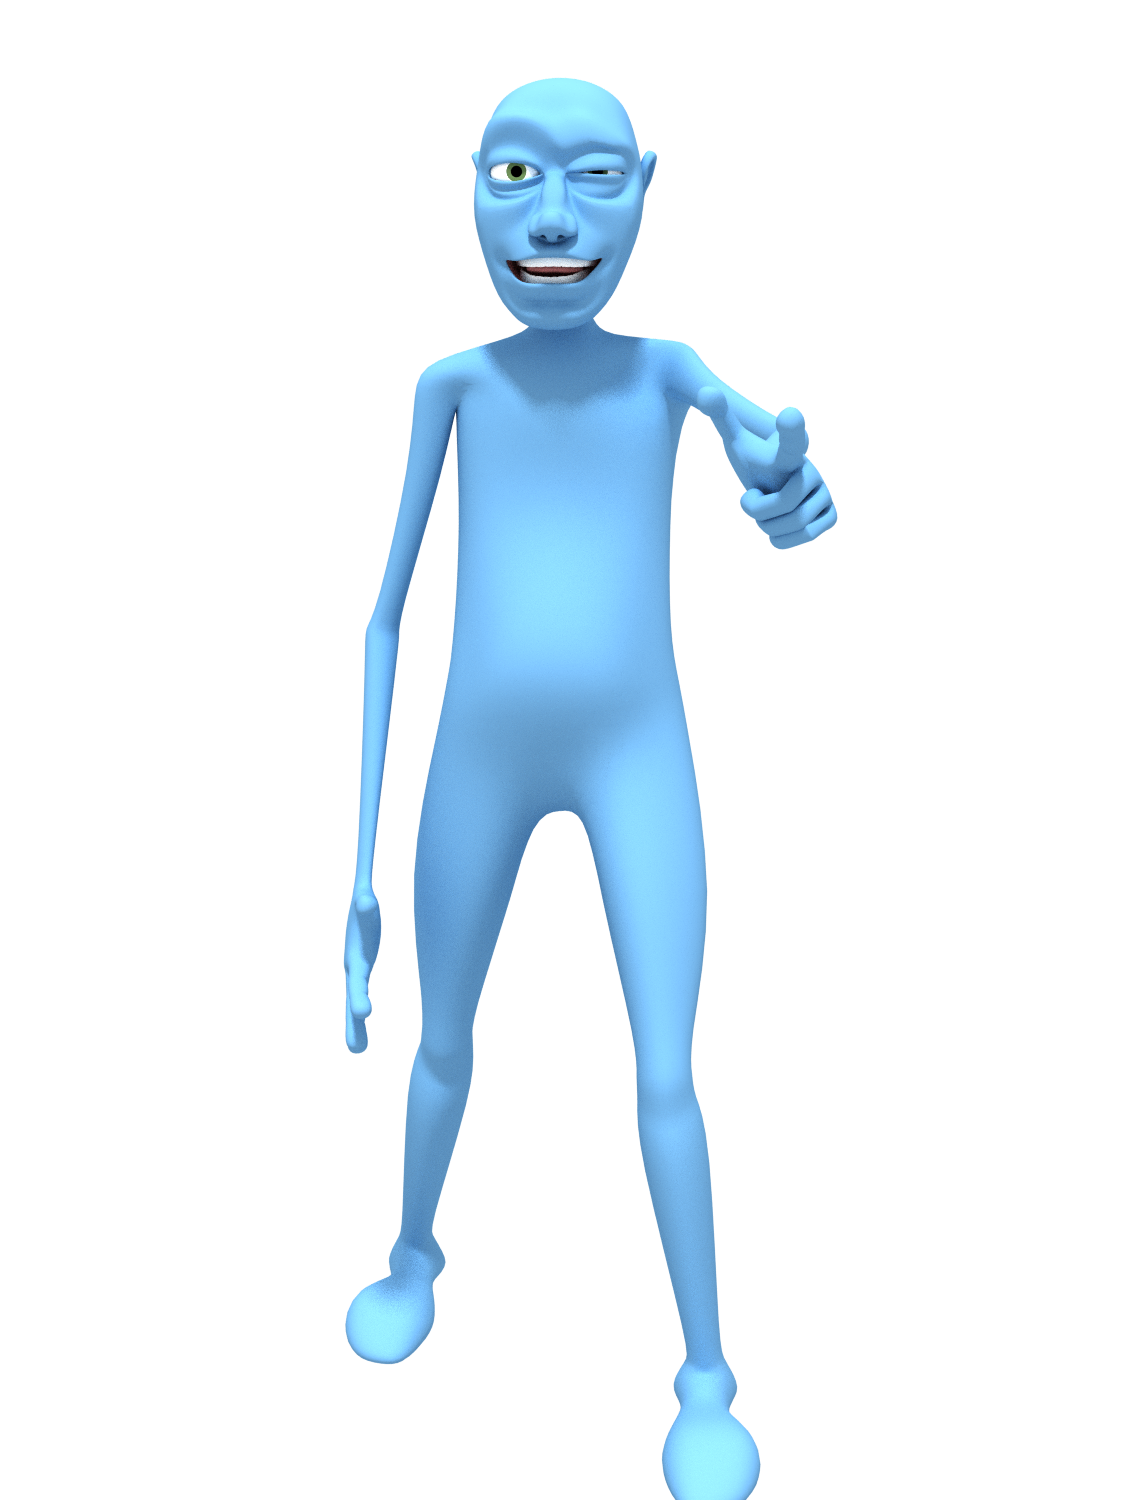
\includegraphics[width=0.8\linewidth]{chapter4/ludwig}
  \caption{}
  \label{fig:ludwig}
\end{subfigure}%
\begin{subfigure}[b]{.5\textwidth}
 \captionsetup{width=0.8\textwidth}
  \centering
  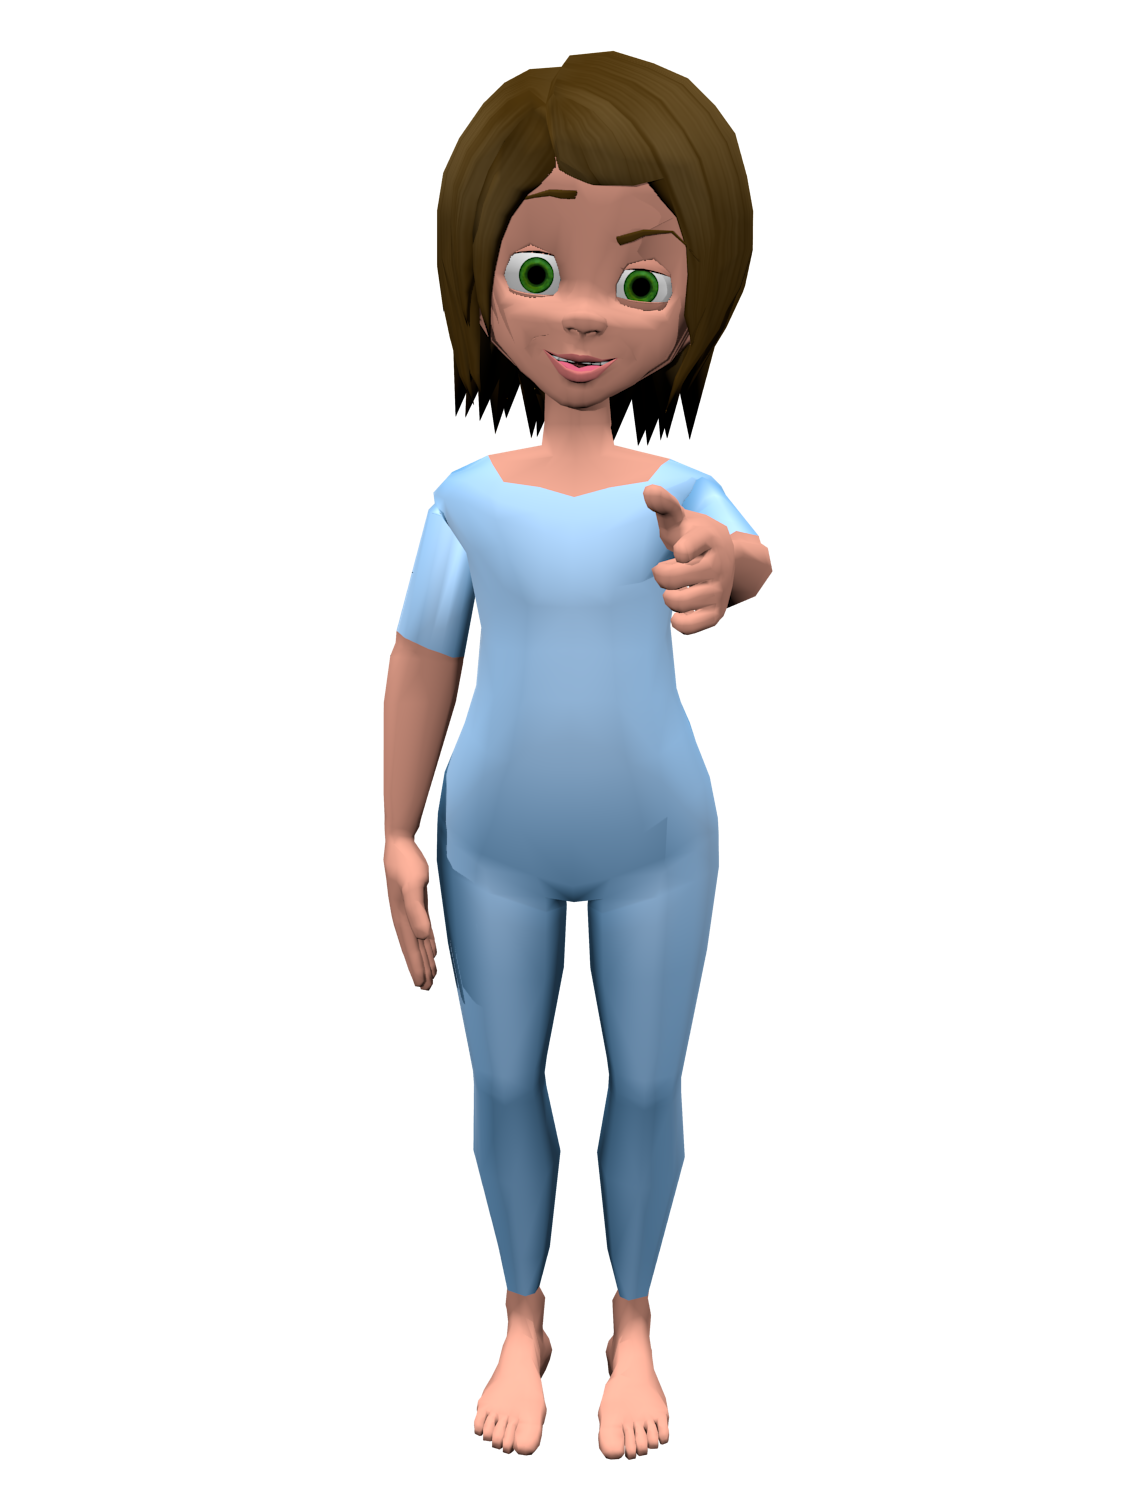
\includegraphics[width=0.8\linewidth]{chapter4/girl}
  \caption{}
  \label{fig:elena}
\end{subfigure}
\caption{Potential 3D avatars - Ludwig and Elena}
\label{fig:models}
\end{figure}

\begin{figure}[H]
	\centering
    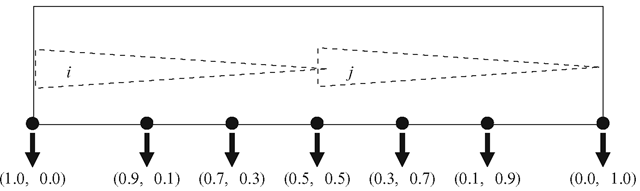
\includegraphics[scale=0.5]{chapter4/weights}
    \caption[A visualisation of the weight falloff]{A visualisation of the weight falloff; from \url{http://what-when-how.com}}
    \label{fig:weights}
\end{figure}	

\begin{figure}[H]
	\centering
    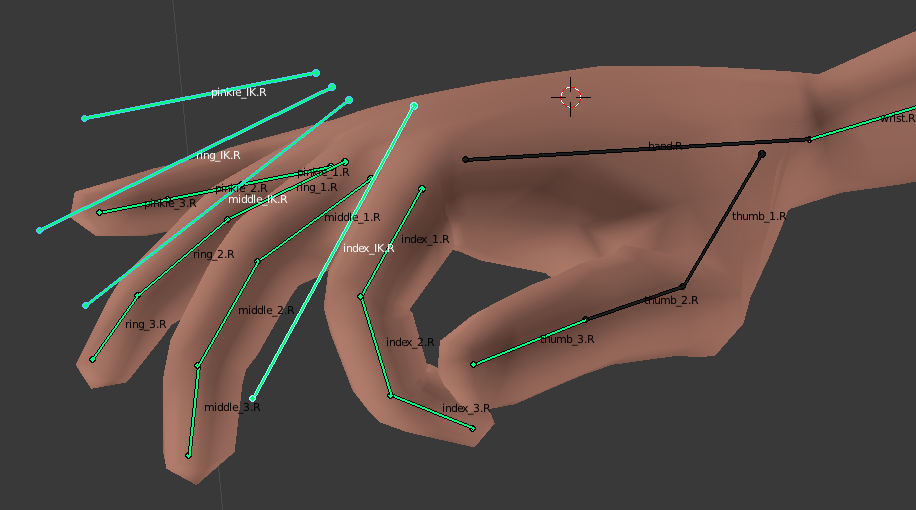
\includegraphics[scale=0.4]{chapter4/hand-zoom}
    \caption[Close up of the avatar hand and underlying bones]{Close up of the avatar hand and underlying bones. In light-blue are IK finger bones.}
    \label{fig:hand}
\end{figure}	
\begin{figure}[H]
\centering
\begin{subfigure}[b]{.6\textwidth}
	\captionsetup{width=0.8\textwidth}
  \centering
  \raisebox{5mm}{
  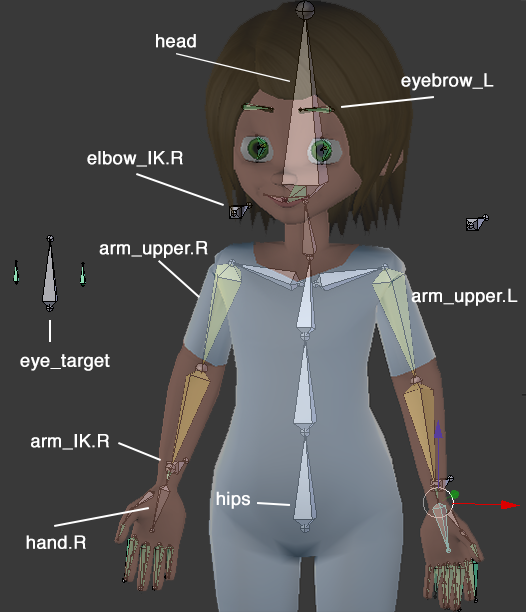
\includegraphics[width=0.8\linewidth]{chapter4/bone-struct}
  }
  \caption{}
\end{subfigure}%
\begin{subfigure}[b]{.6\textwidth}
 \captionsetup{justification=justified, width=0.5\textwidth}
\footnotesize
\begin{minipage}[t]{0.5\linewidth}
\dirtree{%
.1 Pose.
	.2 hips.
		.3 spine\_01.
			.4 spine\_02.
				.5 neck.
					.6 head.
			.4 shoulder\_L.
				.5 arm\_upper.
					.6 arm\_lower.
						.7 wrist.
							.8 hand.
								.9 thumb.
								.9 index.
								.9 middle.
								.9 ring.
								.9 pinkie.
			.4 shoulder-R.
				.5 \textcolor{red}{as above}.
	.2 eye-target.
}
\end{minipage}
  \caption{}
\end{subfigure}
\caption{3D model bone structure}
\label{fig:struct}
\end{figure}

\begin{figure}[H]
	\centering
    \includegraphics[scale=0.9]{chapter4/bezier}
    \caption[Bezier vs. Linear interpolation]{Bezier vs. Linear interpolation. The XYZ axis represents the values of each axis in 3D space.}
    \label{fig:bezier}
\end{figure}	

\begin{figure}[H]
	\centering
    \includegraphics[scale=1]{chapter4/webgl}
    \caption{WebGL rendering pipeline}
    \label{fig:webgl}
\end{figure}	

\begin{figure}[H]
	\centering
    \includegraphics[scale=0.7]{chapter4/concurrent-feats}
    \caption{A BSL sentence and visualised non-manual sequence}
    \label{fig:concurrent-feats}
\end{figure}	

\begin{figure}[H]
	\centering
    \includegraphics[scale=0.75]{chapter4/system-overview-flask}
    \caption{System outline: Flask Framework highlighted}
    \label{fig:sys-over-flask}
\end{figure}	

\begin{figure}[H]
	\centering
    \includegraphics[scale=0.77]{chapter5/wer-example1}
    \caption[WER operations]{WER operations; green lines show correct alignments, and red lines incorrect alignments.}
    \label{fig:wer1}
\end{figure}	

\begin{figure}[H]
	\centering
    \includegraphics[scale=0.77]{chapter5/wer-example2}
    \caption{WER operations on a classifier predicate sentence}
    \label{fig:wer2}
\end{figure}	

\definecolor{bblue}{HTML}{3399FF}
\definecolor{rred}{HTML}{EF3D2A}
\definecolor{yyellow}{HTML}{FDA94E}
\definecolor{ggreen}{HTML}{22C91D}
\definecolor{ppurple}{HTML}{E200E6}

\begin{figure}[H]
\begin{tikzpicture}
    \begin{axis}[
        width  = \textwidth-1cm,
        height = 8cm,
        major x tick style = transparent,
        axis lines*=left,
        ybar=\pgflinewidth,
        bar width=14pt,
        ymajorgrids = true,
        ylabel = {Number of Users},
        %symbolic x coords={Mac,Windows,Linux, iPhone, Android},
        xticklabels =
	    {
	        \strut  Mac,     %% you need comma (,) at the end here and next 2 lines
	        \strut  Windows,
	        \strut  Linux,
	        	\strut  iPhone,
	        	\strut  Android,
	    },
        xtick = {1,2,3,4,5},
        scaled y ticks = false,
        enlarge x limits=0.25,
        ymin=0,
        legend cell align=left,
%        legend style={
%                at={(1,1.05)},
%                anchor=south east
%                column sep=1ex
%        },
		legend style={draw=none, legend columns=-1, column sep=1ex, at={(1,1.1)}},
		nodes near coords
    ]
        \addplot[style={bblue,fill=bblue!50,mark=none}]
            coordinates {(1, 7) (4, 1)};

        \addplot[style={rred,fill=rred!50,mark=none}]
             coordinates {(1, 3) (2, 7) (3, 4) (5, 5)};
             
		\addplot[style={yyellow,fill=yyellow!50,mark=none}]
             coordinates {(1, 2) (2, 3) (3, 3)};

        \addplot[style={ggreen,fill=ggreen!50,mark=none}]
             coordinates {(2, 1)};
             
        \legend{Safari, Chrome, Firefox, Opera, Internet Explorer}
    \end{axis}
\end{tikzpicture}
\caption{Devices and browsers running the website}
\label{fig:devices}
\end{figure}

\def\angle{-45}
\def\radius{2}
\def\cyclelist{{"bblue","rred","ggreen", "yyellow", "ppurple"}}
\newcount\cyclecount \cyclecount=-1
\newcount\ind \ind=-1

\begin{figure}[H]
\centering
\begin{subfigure}[b]{.5\textwidth}
	\captionsetup{width=0.8\textwidth}
  \small
  \centering
  \begin{tikzpicture}
  \foreach \percent/\name in {
  	  62.8/Agree,
  	  32.6/Strongly agree,
	  4.7/Neither agree or disagree
    } {
      \ifx\percent\empty\else               % If \percent is empty, do nothing
        \global\advance\cyclecount by 1     % Advance cyclecount
        \global\advance\ind by 1            % Advance list index
        \ifnum3<\cyclecount                 % If cyclecount is larger than list
          \global\cyclecount=0              %   reset cyclecount and
          \global\ind=0                     %   reset list index
        \fi
        \pgfmathparse{\cyclelist[\the\ind]} % Get color from cycle list
        \edef\color{\pgfmathresult}         %   and store as \color
        % Draw angle and set labels
        \draw[fill={\color!50},draw={\color}] (0,0) -- (\angle:\radius)
          arc (\angle:\angle+\percent*3.6:\radius) -- cycle;
        \node at (\angle+0.5*\percent*3.6:0.7*\radius) {\percent\,\%};
        \node[pin=\angle+0.5*\percent*3.6:\name]
          at (\angle+0.5*\percent*3.6:\radius) {};
        \pgfmathparse{\angle+\percent*3.6}  % Advance angle
        \xdef\angle{\pgfmathresult}         %   and store in \angle
      \fi
    };
\end{tikzpicture}
  \caption{The UI elements are clear and easy to understand}
  \label{}
\end{subfigure}%
\begin{subfigure}[b]{.5\textwidth}
 \captionsetup{width=0.8\textwidth}
  \centering
  \small
  \def\angle{20}
\newcount\cyclecount \cyclecount=-1
\newcount\ind \ind=-1
  \begin{tikzpicture}
  \foreach \percent/\name in {
  	  60.5/Reasonable,
  	  23.3/Short,
  	  4.7/Very short,
  	  7/Long,
  	  4.7/Too long
    } {
      \ifx\percent\empty\else               % If \percent is empty, do nothing
        \global\advance\cyclecount by 1     % Advance cyclecount
        \global\advance\ind by 1            % Advance list index
        \ifnum4<\cyclecount                 % If cyclecount is larger than list
          \global\cyclecount=0             %   reset cyclecount and
          \global\ind=0                   %   reset list index
        \fi
        \pgfmathparse{\cyclelist[\the\ind]} % Get color from cycle list
        \edef\color{\pgfmathresult}         %   and store as \color
        % Draw angle and set labels
        \draw[fill={\color!50},draw={\color}] (0,0) -- (\angle:\radius)
          arc (\angle:\angle+\percent*3.6:\radius) -- cycle;
        \node at (\angle+0.5*\percent*3.6:0.7*\radius) {\percent\,\%};
        \node[pin=\angle+0.5*\percent*3.6:\name]
          at (\angle+0.5*\percent*3.6:\radius) {};
        \pgfmathparse{\angle+\percent*3.6}  % Advance angle
        \xdef\angle{\pgfmathresult}         %   and store in \angle
      \fi
    };
\end{tikzpicture}  
  \caption{Loading times}
  \label{}
\end{subfigure}
\caption[Visualised data for responses on clarity of the UI and loading times]{Visualised data for responses on clarity of the UI and loading times (43 responses)}
\label{fig:chart1}
\end{figure}

\begin{figure}[H]
\centering
\begin{subfigure}[b]{.5\textwidth}
	\captionsetup{width=0.8\textwidth}
  \small
  \centering
  \begin{tikzpicture}
    \begin{axis}[
        width  = \textwidth-1cm,
        height = 8cm,
        major x tick style = transparent,
        axis lines*=left,
        ybar=\pgflinewidth,
        bar width=14pt,
        ymajorgrids = true,
        ylabel = {Number of Selections},
        %symbolic x coords={Mac,Windows,Linux, iPhone, Android},
        xticklabels =
	    {
	        \strut  V. Unnatural,     %% you need comma (,) at the end here and next 2 lines
	        \strut  Unnatural,
	        \strut  Neutral,
	        	\strut  Natural,
	        	\strut  V. Natural,
	    },
        xtick = {1,2,3,4,5},
        xticklabel style={rotate=35, anchor=north east, inner sep=0mm},
        scaled y ticks = false,
        enlarge x limits=0.25,
        ymin=0,
        legend cell align=left,
%        legend style={
%                at={(1,1.05)},
%                anchor=south east
%                column sep=1ex
%        },
		legend style={draw=none, legend columns=-1, column sep=1ex, at={(1,1.1)}},
		nodes near coords
    ]
        \addplot[style={bblue,fill=bblue!50,mark=none}]
            coordinates {(1, 1) (2, 2) (3, 13) (4, 19) (5, 8)};
    \end{axis}
\end{tikzpicture}
  \caption{Rating of avatar movements}
  \label{fig:rating}
\end{subfigure}%
\begin{subfigure}[b]{.5\textwidth}
 \captionsetup{width=0.8\textwidth}
  \centering
  \small
\begin{tikzpicture}
    \begin{axis}[
        width  = \textwidth-1cm,
        height = 8cm,
        major x tick style = transparent,
        axis lines*=left,
        ybar=\pgflinewidth,
        bar width=14pt,
        ymajorgrids = true,
        ylabel = {Number of Selections (29 responses)},
        %symbolic x coords={Mac,Windows,Linux, iPhone, Android},
        xticklabels =
	    {
	        \strut  Gender,     %% you need comma (,) at the end here and next 2 lines
	        \strut  Colours,
	        \strut  Body features
	    },
        xtick = {1,2,3,4,5},
        xticklabel style={rotate=35, anchor=north east, inner sep=0mm},
        scaled y ticks = false,
        enlarge x limits=0.25,
        ymin=0,
        legend cell align=left,
%        legend style={
%                at={(1,1.05)},
%                anchor=south east
%                column sep=1ex
%        },
		legend style={draw=none, legend columns=-1, column sep=1ex, at={(1,1.1)}},
		nodes near coords
    ]
        \addplot[style={ggreen,fill=ggreen!50,mark=none}]
            coordinates {(1, 23) (2, 19) (3, 4)};
    \end{axis}
\end{tikzpicture}
  \caption{Additional customisations}
  \label{fig:custom}
\end{subfigure}
\caption[Movement ratings and avatar customisation]{Movement ratings and avatar customisation including skin and hair colour, avatar height etc.}
\end{figure}

\begin{figure}[H]
\centering
\begin{subfigure}{.47\textwidth}
  \centering
  \Tree [.ROOT
        [.SBARQ
          [.WHADVP [.WRB How ] ]
          [.SQ [.VBP are ] [.NP [.PRP you ] ] ] ] ]
\end{subfigure}%
{\LARGE$\rightarrow$}%
\begin{subfigure}{.47\textwidth}
  \centering
  \Tree [.ROOT
        [.SBARQ
          [.WHADVP [.\textcolor{red}{?} how-are-you ] ]
          [.SQ [.VBP \vphantom{A}$\nothing$ ] [.NP [.PRP \vphantom{A}$\nothing$ ] ] ] ] ]
\end{subfigure}
\caption{Issue with using SignBank before tree transformations}
\label{fig:combined}
\end{figure}

\begin{figure}[H]
\centering
\begin{subfigure}[b]{.5\textwidth}
	\captionsetup{width=0.8\textwidth}
  \centering
  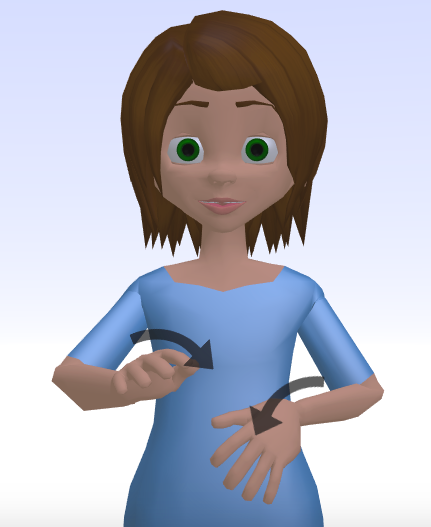
\includegraphics[width=0.7\linewidth]{chapter6/animal2}
  \caption{}
\end{subfigure}%
\begin{subfigure}[b]{.5\textwidth}
 \captionsetup{width=0.8\textwidth}
  \centering
  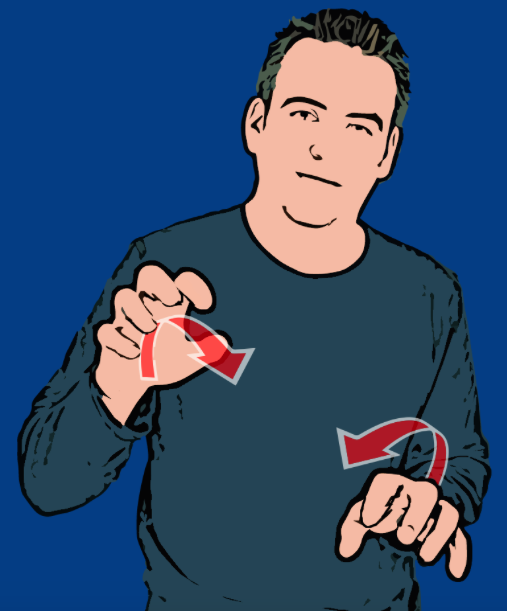
\includegraphics[width=0.7\linewidth]{chapter6/animal1}
  \caption{}
\end{subfigure}
\label{fig:storyboard}
\end{figure}

\begin{figure}[H]
	\centering
    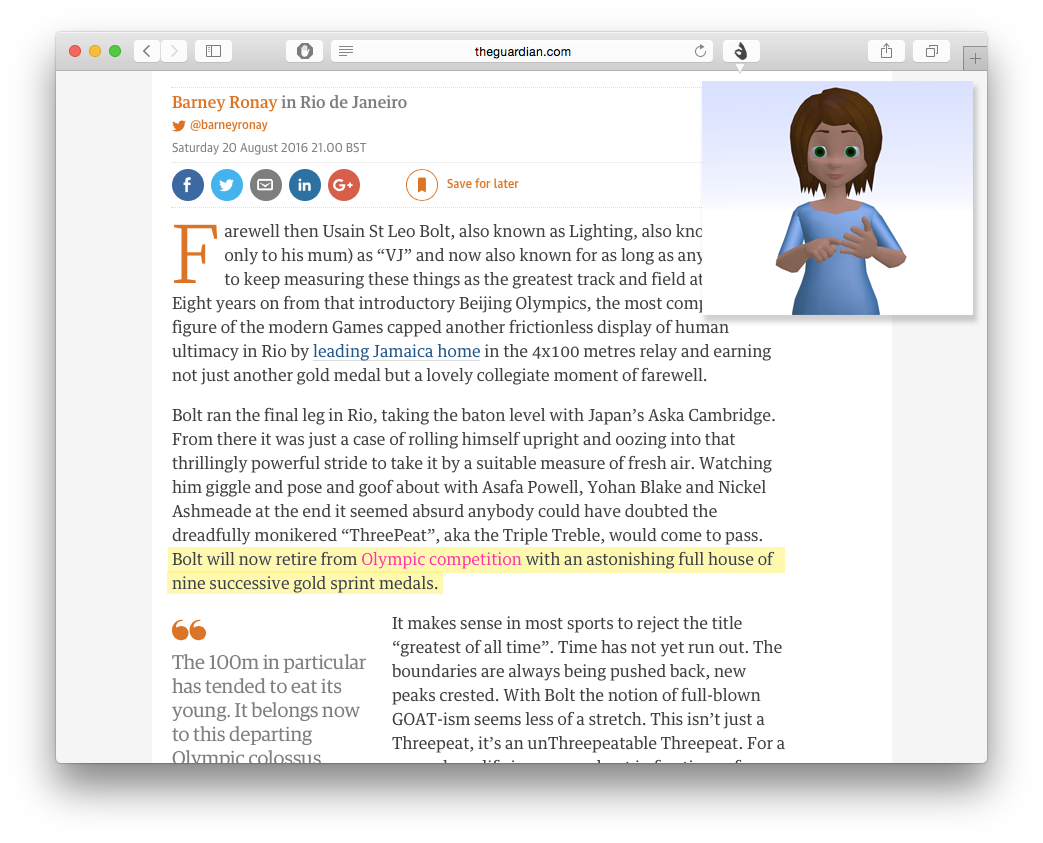
\includegraphics[scale=0.35]{chapter6/concept}
    \caption[Possible browser add-on for the current system]{Possible browser add-on for the current system. The current sentence is highlighted in yellow and the words being signed (approximated) are coloured in pink.}
    \label{fig:concept}
\end{figure}	

\begin{figure}[h]
	\centering
	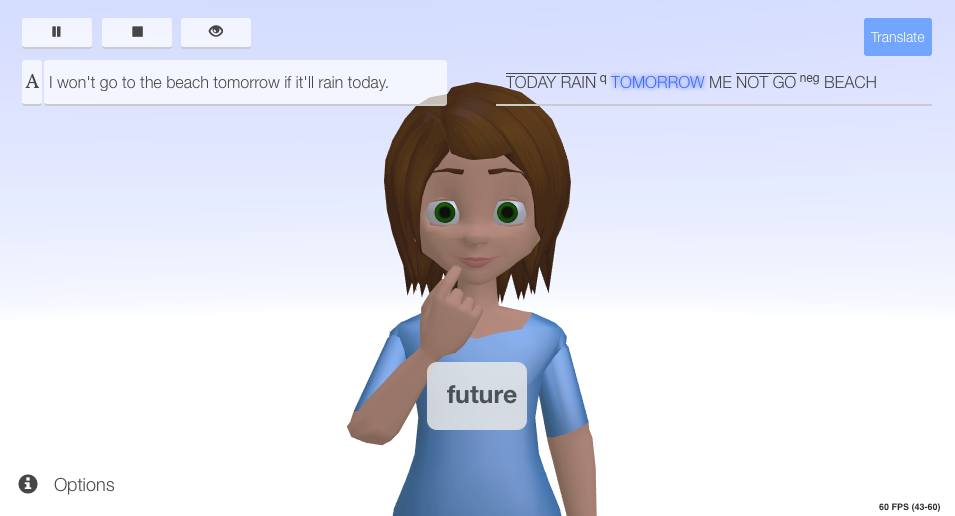
\includegraphics[scale=0.4]{appendix/future}
    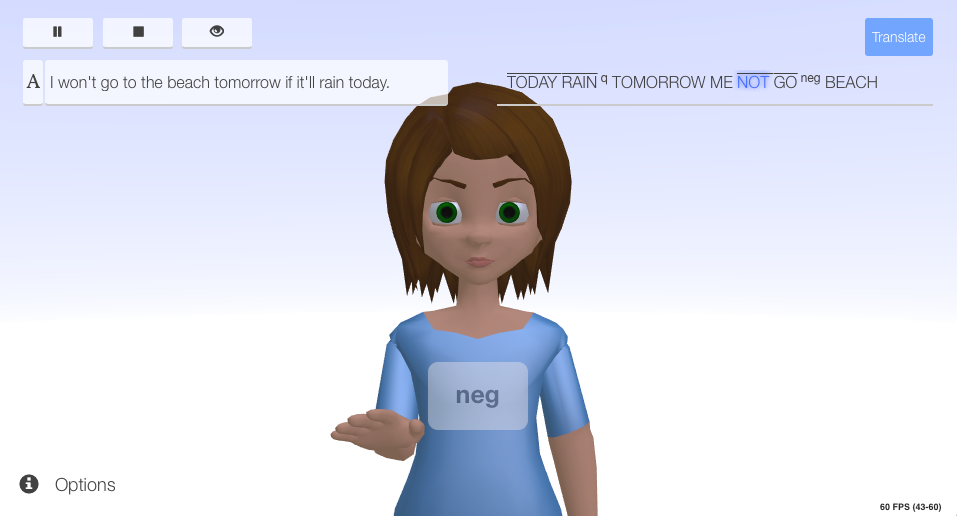
\includegraphics[scale=0.4]{appendix/neg}
    \caption{``Show non-manual features'' enabled playback}
    \label{fig:non-man-app}
\end{figure}	

\begin{figure}[h]
	\centering
    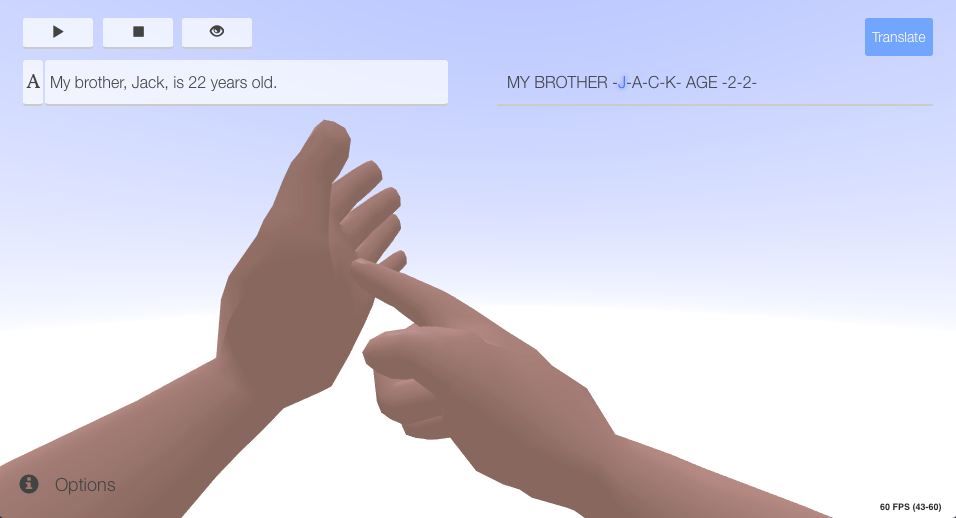
\includegraphics[scale=0.45]{appendix/fpv}
    \caption{First person view of the avatar when fingerspelling the letter ``J''}
    \label{fig:fpv}
\end{figure}
\begin{figure}[h]
	\centering
    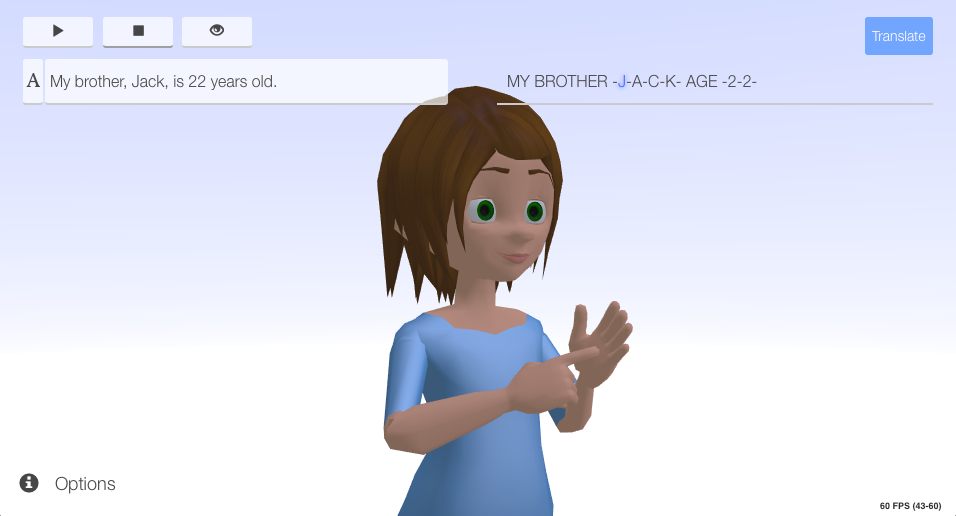
\includegraphics[scale=0.45]{appendix/3rd}
    \label{fig:3rd}
\end{figure}

\end{document}